\documentclass[./main.tex]{subfiles}

\usetikzlibrary{matrix}
\usepackage{bm}

\begin{document}
    \ExamQuestion{問2}
    % \subsubsection*{問2}
    % \addcontentsline{toc}{subsubsection}{問2}
    % \markboth{2025年 統計応用 理工学 問2}{2025年 統計応用 理工学 問2}

    \begin{enumerate}
        % Q1
        \item $\mathrm{A} \xrightarrow{0.95} \mathrm{A} \xrightarrow{0.95} \mathrm{A}$ という推移の確率を求めて,
            $0.95^2 = 0.9025.$
        
        % Q2
        \item 以下のような推移の確率を求めて, 
        $3 \cdot 0.95^2 \cdot 0.04 = 0.1083.$

        \begin{figure}[h]
            \centering
            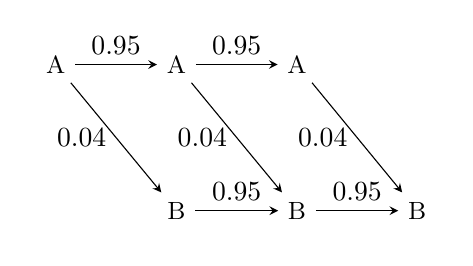
\begin{tikzpicture}
                \matrix (m) [matrix of nodes, 
                    row sep=4em, column sep=3em,
                    minimum width=1em,
                    nodes={font=\small}] 
                {
                    A & A & A &  \\
                      & B & B & B\\
                };
                \path[-stealth]
                (m-1-1) edge node[above] {0.95} (m-1-2)
                        edge node[left] {0.04} (m-2-2)
                (m-1-2) edge node[above] {0.95} (m-1-3)
                        edge node[left] {0.04} (m-2-3)
                (m-1-3) edge node[left] {0.04} (m-2-4)
                (m-2-2) edge node[above] {0.95} (m-2-3)
                (m-2-3) edge node[above] {0.95} (m-2-4);
            \end{tikzpicture}
        \end{figure}

        % Q3
        \item 状態ベクトル $\bm{e}_1$ を 10 回推移させたものの第 3 成分が答えであり, 
            $\bm{e}_1^T P^{10} \bm{e}_3.$


        \item
    \end{enumerate}
    \newpage\newpage
\end{document}